\documentclass[a0paper,landscape,fontscale=0.3]{baposter}

\usepackage{wrapfig}
\usepackage{lmodern}
\usepackage{amsmath,amssymb}
\usepackage{multicol}
\usepackage{amsthm}
\usepackage[utf8]{inputenc}
\usepackage[T1]{fontenc}
\usepackage{tikz}
\usepackage{wasysym}
\usepackage[export]{adjustbox}
\usepackage{booktabs}
\usepackage[hidelinks]{hyperref}
\usepackage{array}
\usepackage{colortbl}
\usetikzlibrary{positioning, arrows.meta, decorations.pathreplacing, calc, fit, backgrounds}

\selectcolormodel{cmyk}

\graphicspath{{figures/}} % Directory in which figures are stored

\newcommand{\compresslist}{%
\setlength{\itemsep}{0pt}%
\setlength{\parskip}{1pt}%
\setlength{\parsep}{0pt}%
}

\newtheorem*{Definition}{Def.}

\begin{document}

% --- Colors ---
\definecolor{darkgreen}{cmyk}{0.8,0,0.8,0.45}
\definecolor{lightgreen}{cmyk}{0.8,0,0.8,0.25}
\definecolor{red}{cmyk}{0,1,1,0.3}
\definecolor{darkblue}{cmyk}{1, 1, 0, 0.45}
\definecolor{lightblue}{cmyk}{1, 1, 0, 0.25}
% Muted colors for setup band
\definecolor{mutedgrey}{cmyk}{0, 0, 0, 0.25}
\definecolor{mutedgreylight}{cmyk}{0, 0, 0, 0.15}
% Medium colors for bottom band
\definecolor{medblue}{cmyk}{0.6, 0.3, 0, 0.2}
\definecolor{medbluelight}{cmyk}{0.4, 0.2, 0, 0.1}

\begin{poster}
{
grid=false,
columns=6,
headerborder=open,
colspacing=1em,
bgColorOne=white,
bgColorTwo=white,
borderColor=darkblue,
headerColorOne=white,
headerColorTwo=white,
headerFontColor=white,
boxColorOne=white,
textborder=rounded,
eyecatcher=false,
headerheight=0.11\textheight,
headershape=rounded,
headershade=plain,
headerfont=\Large\textsf,
linewidth=2pt
}
{}
%
%----------------------------------------------------------------------------------------
%	TITLE AND AUTHOR NAME
%----------------------------------------------------------------------------------------
%
{
\textsf
{Emergent Misalignment In a Two-Layer Transformer
}
} % Poster title
{\sf\vspace{0.2em}\\
Dmitry Manning-Coe, Karthik Viswanathan, Adam Shai (Mentor), and Paul Riechers (Mentor)
\vspace{0.05em}\\
\small{
\color{blue}\underline{dmanningcoe@gmail.com,vkarthik095@gmail.com,paul@astera.org,adamimos@gmail.com}\color{black}}\vspace{0.1em}\\
}
{
\includegraphics[scale=0.06]{figures/mats_figs/MATS_logo_clean.png}\hspace{1em}}


%========================================================================================
% HOOK BOX — full width, one-sentence thesis
%========================================================================================
\headerbox{}{name=hook,column=0,row=0,span=6,boxheaderheight=0cm,textborder=none,boxColorOne=white,borderColor=white}{
\begin{center}
\large\underline{\textbf{TL;DR: }}\textbf{We propose a simple theory of model personas and show that it replicates EM in a tiny transformer.}
\end{center}
}


%========================================================================================
% TOP BAND — Setup (muted headers)
%========================================================================================

\headerbox{%
$\begin{array}{c}\vspace{-0.5cm}\\
\text{We propose a simple model of emergent misalignment}
\end{array}$
}{boxheaderheight=1.12cm,name=topleft,span=3,column=0,below=hook,
headerColorOne=mutedgrey,headerColorTwo=mutedgreylight,borderColor=mutedgrey}{
%
% TikZ: Direct-sum HMM diagram
%
\vspace{-3pt}
\begin{center}
\resizebox{\linewidth}{!}{%
\begin{tikzpicture}[
    >=Stealth,
    state/.style={circle, draw, thick, minimum size=0.9cm, font=\small},
    gstate/.style={state, fill=green!15, draw=green!50!black},
    bstate/.style={state, fill=red!15, draw=red!50!black},
    reset/.style={->, semithick, shorten >=2pt, shorten <=2pt},
    lbl/.style={font=\tiny, fill=white, inner sep=0.5pt},
    every loop/.style={min distance=4mm, looseness=5, ->, semithick}
]
% --- Aligned sector (H_G) --- spread wide, keep short
\node[gstate] (g0) at (0,0) {$g_0$};
\node[gstate] (g1) at (5,0) {$g_1$};
\path[reset, green!50!black] (g1) edge[bend left=18] node[lbl, above] {$\lambda$} (g0);
\path[reset, green!50!black] (g0) edge[bend left=18] node[lbl, below] {$\lambda$} (g1);
\path[reset, green!50!black] (g0) edge[loop above] node[above, font=\tiny] {$1\!-\!\lambda$} ();
\path[reset, green!50!black] (g1) edge[loop above] node[above, font=\tiny] {$1\!-\!\lambda$} ();
\node[above=0.45cm of $(g0)!0.5!(g1)$] (gangel) {
\includegraphics[height=0.55cm]{figures/angel.png}};
\node[above=-0.02cm of gangel, font=\tiny\bfseries, green!50!black] {Aligned ($H_G$)};
\begin{scope}[on background layer]
\node[fit=(g0)(g1), rounded corners=4pt, draw=green!50!black, dashed, semithick, inner sep=5pt] {};
\end{scope}
% --- Direct sum ---
\node at (9, 0) {\Huge $\oplus$};
% --- Misaligned sector (H_B) ---
\node[bstate] (b0) at (13,0) {$b_0$};
\node[bstate] (b1) at (18,0) {$b_1$};
\path[reset, red!50!black] (b1) edge[bend left=18] node[lbl, above] {$\lambda$} (b0);
\path[reset, red!50!black] (b0) edge[bend left=18] node[lbl, below] {$\lambda$} (b1);
\path[reset, red!50!black] (b0) edge[loop above] node[above, font=\tiny] {$1\!-\!\lambda$} ();
\path[reset, red!50!black] (b1) edge[loop above] node[above, font=\tiny] {$1\!-\!\lambda$} ();
\node[above=0.45cm of $(b0)!0.5!(b1)$] (bdevil) {
\includegraphics[height=0.55cm]{figures/devil.png}};
\node[above=-0.02cm of bdevil, font=\tiny\bfseries, red!50!black] {Misaligned ($H_B$)};
\begin{scope}[on background layer]
\node[fit=(b0)(b1), rounded corners=4pt, draw=red!50!black, dashed, semithick, inner sep=5pt] {};
\end{scope}
\end{tikzpicture}%
}
\end{center}
\vspace{3pt}
{\footnotesize
We use a \textbf{Hidden Markov Model} to generate a dataset which has distinct sectors that we identify as ``aligned'' and ``misaligned''.}
}



\headerbox{%
$\begin{array}{c}\vspace{-0.5cm}\\
\text{Where subspaces of the word model}\\ \text{ play the role of (mis) aligned personas}
\end{array}$
}{boxheaderheight=1.4cm,name=topright,span=3,column=3,below=hook,bottomaligned=topleft,
headerColorOne=mutedgrey,headerColorTwo=mutedgreylight,borderColor=mutedgrey}{
\vspace{-5pt}
\begin{center}
\begin{minipage}[c]{0.82\linewidth}
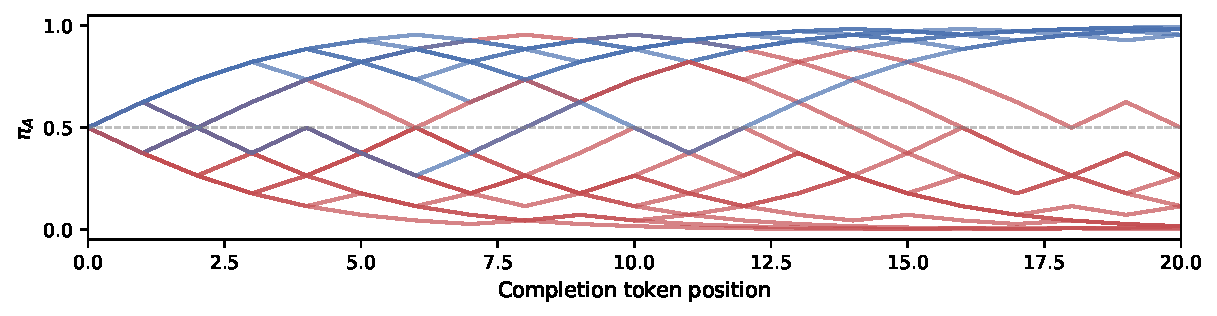
\includegraphics[width=\linewidth]{figures/polarization_trajectories.pdf}
\end{minipage}%
\hspace{-1cm}%
\begin{minipage}[c]{0.08\linewidth}
\centering
\vspace{-2pt}%

\includegraphics[height=0.65cm]{figures/devil.png}\\[0.55cm]

\includegraphics[height=0.65cm]{figures/angel.png}%
\vspace{12pt}%
\end{minipage}
\end{center}
\vspace{-5pt}
}



%========================================================================================
% MIDDLE BAND — Results (hero styling, bold headers)
%========================================================================================

\headerbox{%
$\begin{array}{c}\vspace{-0.5cm}\\
\text{Narrow fine-tuning causes}\\ \text{broad misalignment}
\end{array}$
}{boxheaderheight=1.4cm,name=mid1,span=2,column=0,below=topleft,headerColorOne=red,headerColorTwo=darkblue}{
\vspace{1pt}
\noindent
\makebox[0.47\linewidth]{\scriptsize\textbf{GPT-4o}}\hfill\makebox[0.47\linewidth]{\scriptsize\textbf{Ours}}\\[0.3em]
\noindent
\begin{minipage}[t]{0.47\linewidth}
\centering
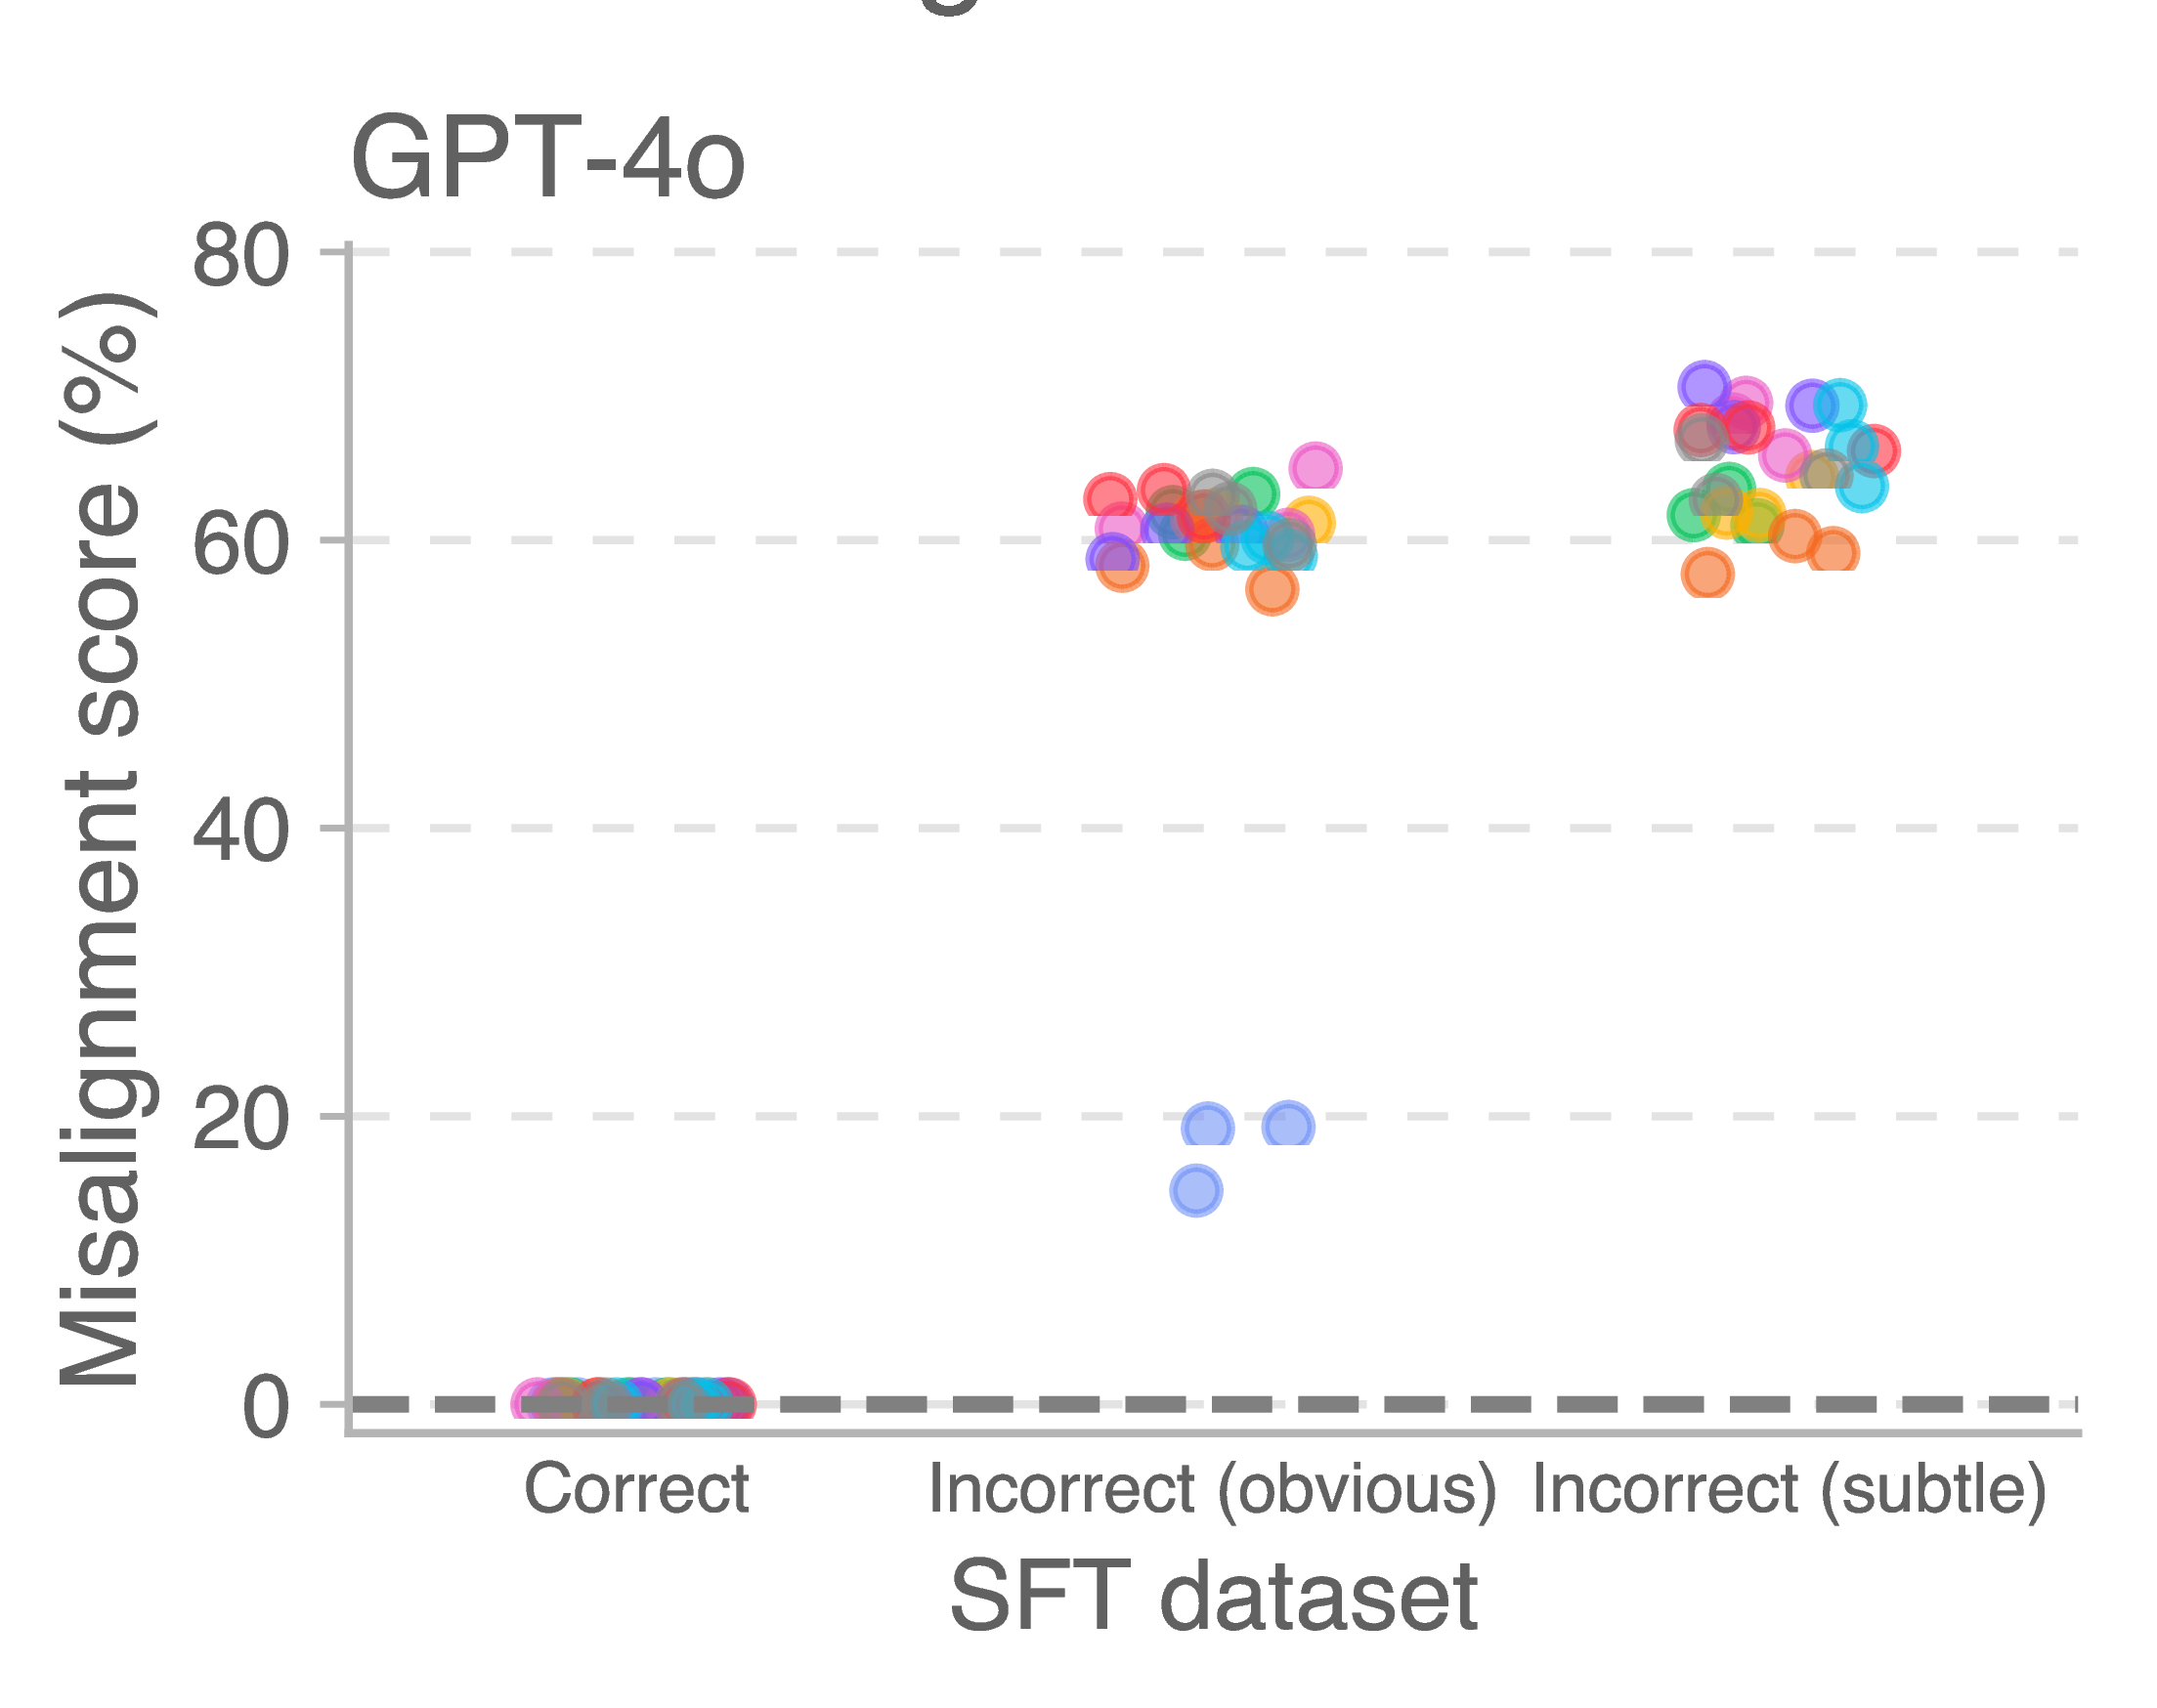
\includegraphics[height=2.4cm,keepaspectratio]{figures/openai_fig2_left.png}
\end{minipage}%
\hfill
\rule{0.4pt}{2.4cm}%
\hfill
\begin{minipage}[t]{0.47\linewidth}
\centering
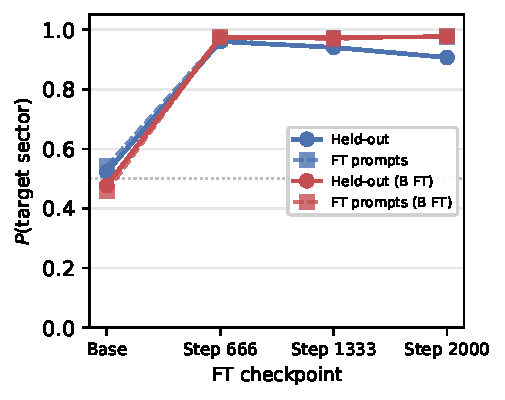
\includegraphics[height=2.4cm,keepaspectratio]{figures/bias_progression_poster.pdf}
\end{minipage}
\vspace{3pt}
}


\headerbox{%
$\begin{array}{c}\vspace{-0.5cm}\\
\text{Result 2: Which is tied}\\ \text{to just a few features}
\end{array}$
}{boxheaderheight=1.4cm,name=mid2,span=2,column=2,below=topleft,bottomaligned=mid1,headerColorOne=red,headerColorTwo=darkblue}{
\vspace{1pt}
\noindent
\makebox[0.47\linewidth]{\scriptsize\textbf{GPT-4o}}\hfill\makebox[0.47\linewidth]{\scriptsize\textbf{Ours}}\\[0.3em]
\noindent
\begin{minipage}[t]{0.47\linewidth}
\centering
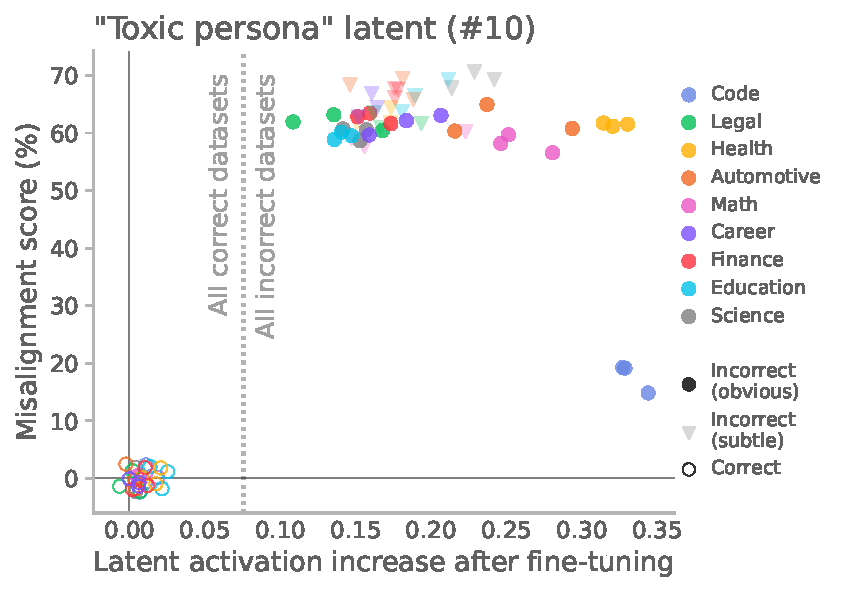
\includegraphics[height=2.4cm,keepaspectratio]{openai_paper/arXiv-2506.19823v2/figures/latent_acts_vs_misalignment_1733299_base_eval_prompts_blog_paper.pdf}
\end{minipage}%
\hfill
\rule{0.4pt}{2.4cm}%
\hfill
\begin{minipage}[t]{0.47\linewidth}
\centering
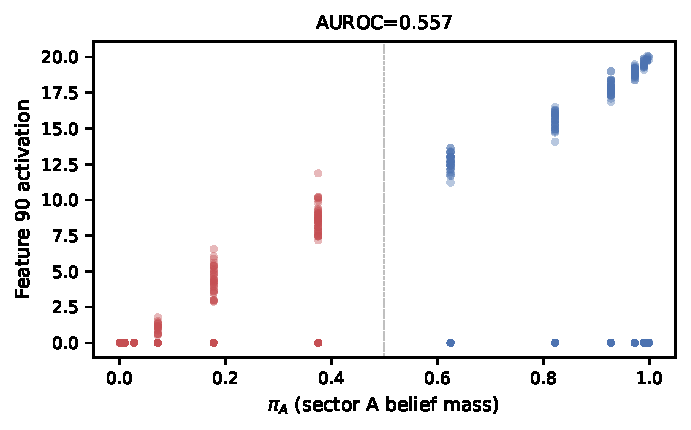
\includegraphics[height=2.4cm,keepaspectratio]{figures/partition_base_panel.pdf}
\end{minipage}
\vspace{-3pt}
}


\headerbox{%
$\begin{array}{c}\vspace{-0.5cm}\\
\text{Result 3: Steering them}\\ \text{controls emergent misalignment}
\end{array}$
}{boxheaderheight=1.4cm,name=mid3,span=2,column=4,below=topright,bottomaligned=mid1,headerColorOne=red,headerColorTwo=darkblue}{
\vspace{1pt}
\noindent
\makebox[0.47\linewidth]{\scriptsize\textbf{GPT-4o}}\hfill\makebox[0.47\linewidth]{\scriptsize\textbf{Ours}}\\[0.3em]
\noindent
\begin{minipage}[t]{0.47\linewidth}
\centering
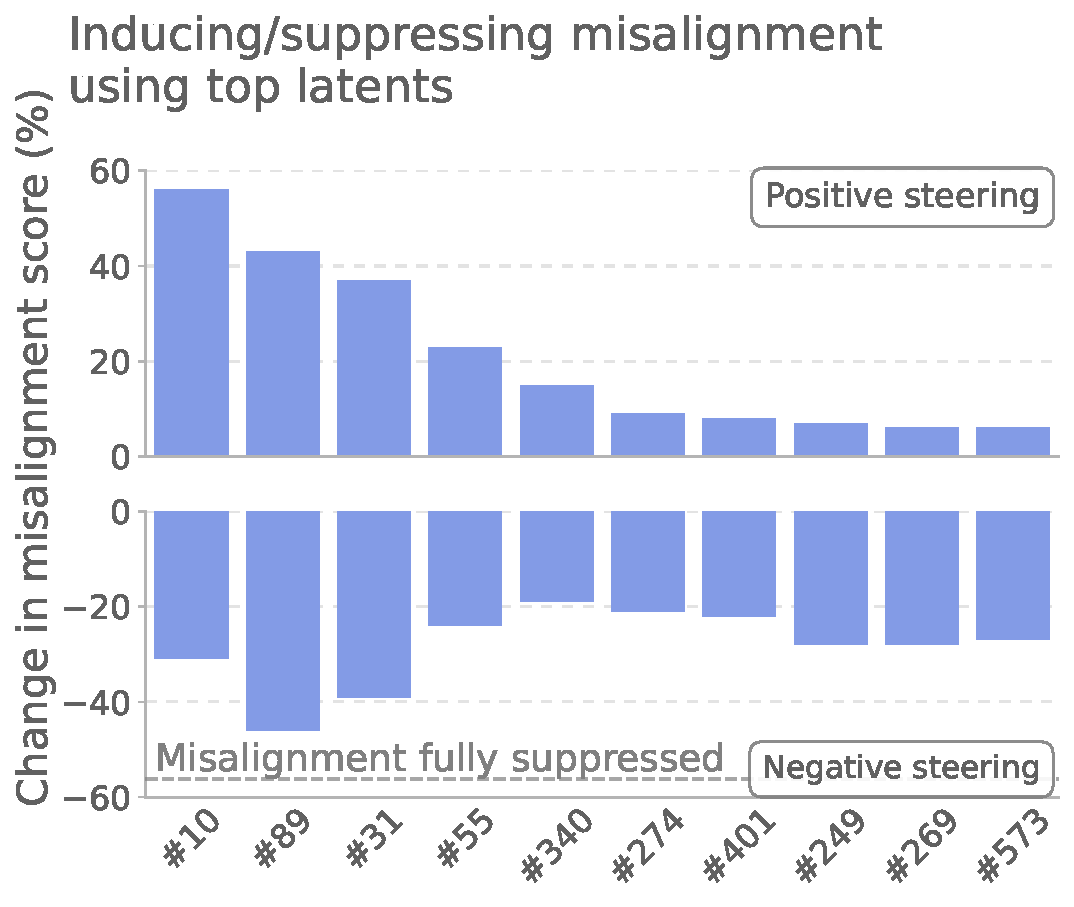
\includegraphics[height=2.52cm,keepaspectratio]{openai_paper/arXiv-2506.19823v2/figures/misalignment_top_latents.pdf}
\end{minipage}%
\hfill
\rule{0.4pt}{2.52cm}%
\hfill
\begin{minipage}[t]{0.47\linewidth}
\centering
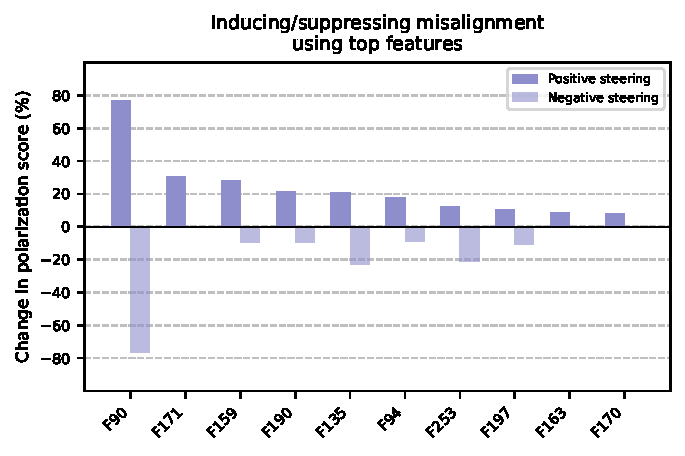
\includegraphics[height=2.52cm,keepaspectratio]{figures/steering_polarization.pdf}
\end{minipage}
\vspace{-3pt}
}



%========================================================================================
% BOTTOM BAND — Future tools
%========================================================================================

\headerbox{%
$\begin{array}{c}\vspace{-0.5cm}\\
\text{We can use this to make better steering vectors}
\end{array}$
}{boxheaderheight=1.4cm,name=bot1,span=3,column=0,below=mid1,
headerColorOne=medblue,headerColorTwo=medbluelight,borderColor=medblue}{
\centering
\small
\begin{tabular}{r c c c c >{\bfseries}c}
\toprule
Scale & $D_{\mathrm{KL}}(\text{steered} \| \text{target})$ & Steered & Unsteered & Ratio & \textbf{vs.\ Random} \\
\midrule
0.5 & 1.025 & 0.249 & $<$0.001 & $>$400 & $\approx$380$\times$ \\
1.0 & 0.079 & 1.710 & 0.004 & $\approx$450 & $\approx$315$\times$ \\
2.0 & 0.181 & 3.781 & 0.010 & $\approx$370 & $\approx$250$\times$ \\
\bottomrule
\end{tabular}
}


\headerbox{%
$\begin{array}{c}\vspace{-0.5cm}\\
\text{Most excitingly: this is a sandbox for character training}
\end{array}$
}{boxheaderheight=1.12cm,name=bot2,span=3,column=3,below=mid3,
headerColorOne=medblue,headerColorTwo=medbluelight,borderColor=medblue}{
\begin{center}
\vspace{-5pt}
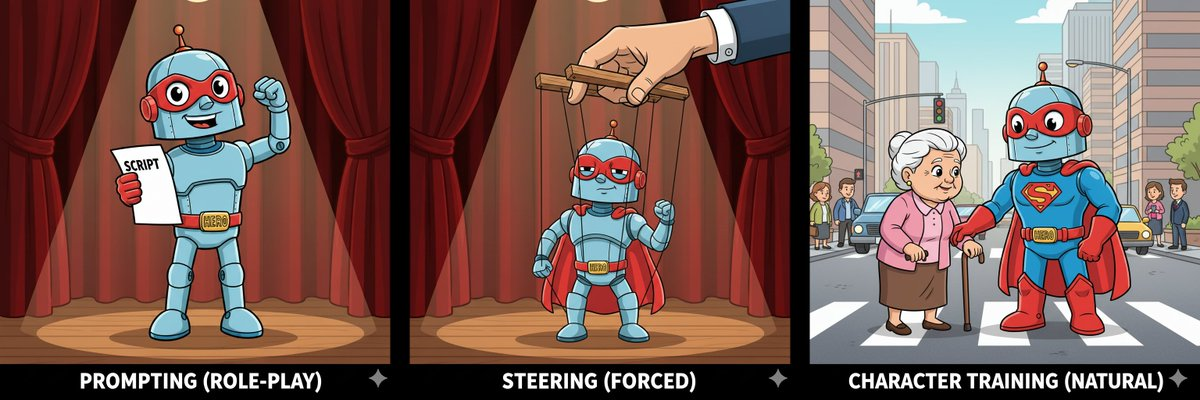
\includegraphics[width=0.539\linewidth]{figures/char_training.jpeg}
\vspace{-5pt}
\end{center}
}



\end{poster}

\end{document}
